\documentclass[12pt]{article}
 
\usepackage[margin=1in]{geometry} 
\usepackage{amsmath,amsthm,amssymb}
\usepackage{graphicx}
\usepackage{attachfile}
\usepackage{multicol}


\graphicspath{ {images/} }
 

\begin{document}
 
% --------------------------------------------------------------
%                         Start here
% --------------------------------------------------------------
 
\title{\Huge \textbf{Tým xhricma00 varianta vv-BVS}}

\author{\bf Marek Hric \\
\bf xhricma00
\and Mikuláš Lešiga\\
 xlesigm00
\and Roman Andraščík \\
 xandrar00
\and Adam Veselý \\ 
xvesela00
}

\maketitle
\bigskip
\begin{center}
 \Large \textbf{Rozdelenie bodov}  \normalsize
 \\ 
\medskip
xhricma00: 25\% \\
xlesigm00: 25\% \\
xandrar00: 25\% \\
xvesela00: 25\%  \\
\bigskip
 \Large \textbf{Rozšírenia} \normalsize
\\
\medskip
ORELSE\\
UNREACHABLE\\
BOOLTHEN\\
FOR\\
WHILE\\
FUNEXP\\
\end{center}

\newpage

\noindent \Large \textbf{Rozdelenie prace :} \\
\noindent\makebox[\linewidth]{\rule{\textwidth}{0.4pt}}
\newline \\
\large Marek Hric : 
\normalsize
\begin{itemize}
\item Lexikálna analýza
\item Generovanie kodu
\end{itemize}
\large Mikuláš Lešiga :
\normalsize
\begin{itemize}
\item Syntaktická analýza bez výrazov
\item Semantická analýza bez výrazov
\item LL Gramatika
\item LL tabuľka, precedenčná tabuľka
\end{itemize}
\large Roman Andraščík :
\normalsize
\begin{itemize}
\item Testy
\item Pomocné funkcie
\item Symtable
\item Dokumentácia
\end{itemize}
\large Adam Veselý :
\normalsize
\begin{itemize}
\item Syntaktická analýza - výrazy
\item Semantická analýza - výrazy
\item Dátové štruktúry
\end{itemize}
 
\newpage

\noindent \Large \textbf{Diagram konečného automatu :}
\newline \\
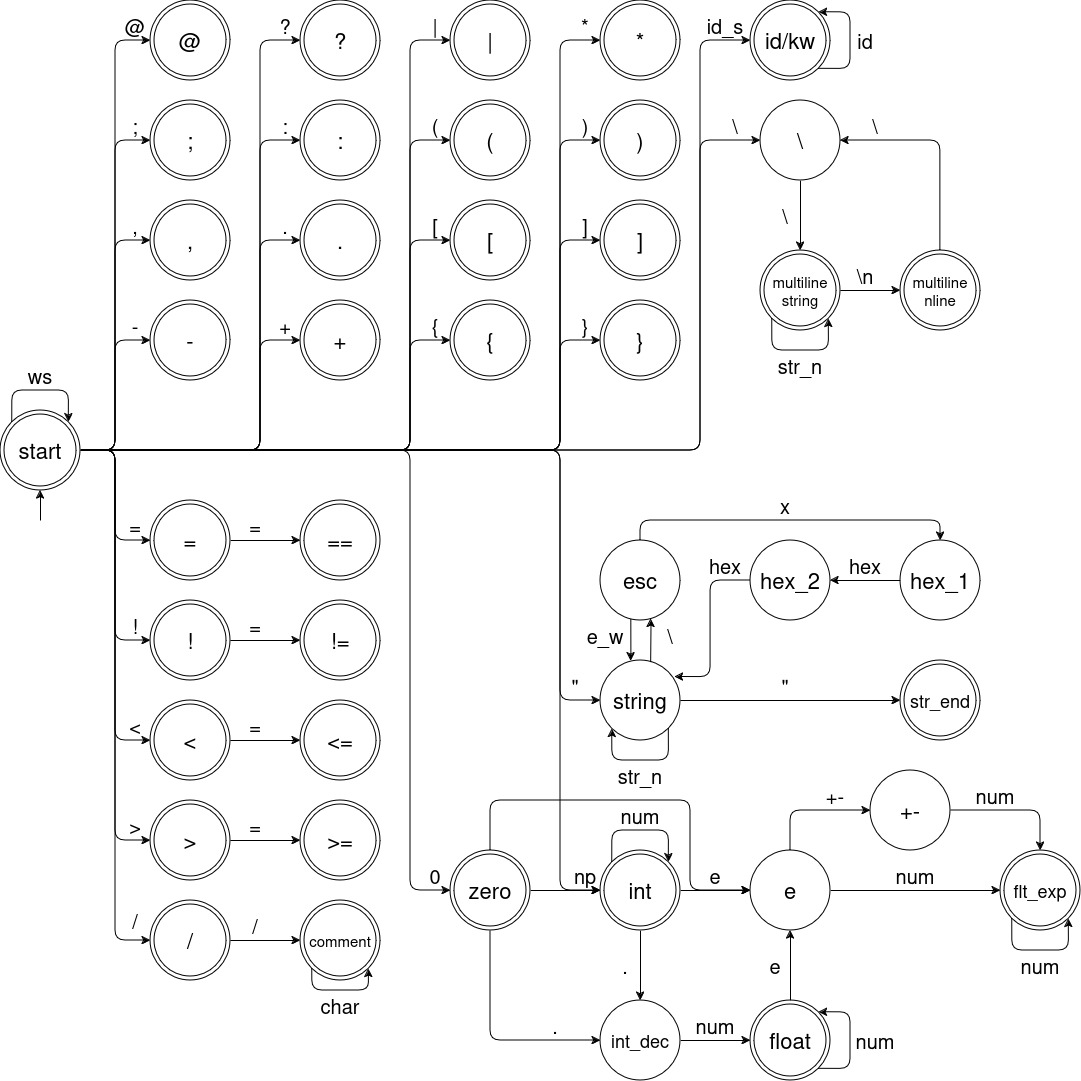
\includegraphics[width=0.8\textwidth,scale=0.5]{fsm}
\newline \\

\textbf{Legenda:}
\small
\begin{multicols}{2}
\begin{itemize}
\item \textbf{ws} - white space
\item \textbf{id\_s} - znaky začiatku identifikátora (\_a-zA-Z)
\item \textbf{id} - znaky identifikátora (\_a-zA-Z0-9)
\item \textbf{num} - čísla (0-9)
\item \textbf{np} - čísla bez nuly (1-9)
\item \textbf{hex} - hexa čísla (0-9a-fA-F)
\item \textbf{e} - exponent (eE)
\item \textbf{char} - ľubovolný znak
\item \textbf{e\_w} - znaky escape sekvencii bez x (n,t,r)
\item \textbf{str\_n} - ľubovolný znak bez $\backslash n$
\end{itemize}
\end{multicols}



\newpage

 \Large \textbf{LL-gramatika :} \\ \normalsize
\noindent\makebox[\linewidth]{\rule{\textwidth}{0.4pt}}

\begin{enumerate}
\item $<prog>\text{ }\to \text{ }<prolog> <function\_def> <end>$
\item $<prolog> \text{ }\to \text{ const ID} = @import ( <expression> ) ;$
\item $<end> \text{ }\to \text{ } EOF$
\item $<function\_def> \text{ }\to \text{ pub fn ID}  (<param\_list>) <function\_type> <block> <function\_def>$
\item $<function\_def> \text{ }\to \text{ } \varepsilon$
\item $<param\_list> \text{ }\to \text{ } ID : <type\_complete> <comma\_par\_found>$
\item $<param\_list> \text{ }\to \text{ } \varepsilon$
\item $<comma\_par\_found> \text{ }\to \text{ } , <param\_list>$
\item $<comma\_par\_found> \text{ }\to \text{ } \varepsilon$
\item $<block> \text{ }\to \text{ } \{ <statement> \}$
\item $<statement> \text{ }\to \text{ } <var\_declaration> <statement>$
\item $<statement> \text{ }\to \text{ } ID <ID\_found> <statement>$
\item $<statement> \text{ }\to \text{ } <if\_statement> <statement>$
\item $<statement> \text{ }\to \text{ } <for\_loop> <statement>$
\item $<statement> \text{ }\to \text{ } <while\_loop> <statement> $
\item $<statement> \text{ }\to \text{ } <return\_statement> <statement>$
\item $<statement> \text{ }\to \text{ } <break> <statement>$
\item $<statement> \text{ }\to \text{ } <continue> <statement>$
\item $<statement> \text{ }\to \text{ } \varepsilon$
\item $<ID\_found> \text{ }\to \text{ } = <asgn\_found> ;$
\item $<ID\_found> \text{ }\to \text{ } ( <expression\_list> );$
\item $<ID\_found> \text{ }\to \text{ } : <while\_loop>$
\item $<var\_declaration> \text{ }\to \text{ const ID} : <type\_complete> = <asgn\_found> ;$
\item $<var\_declaration> \text{ }\to \text{ var ID} : <type\_complete> = <asgn\_found> ;$
\item $<if\_statement> \text{ }\to \text{ } if ( <expression> ) <if\_found>$
\item $<if\_found> \text{ }\to \text{ } <optional\_value> <block> <else\_statement>$
\item $<else\_statement> \text{ }\to \text{ } else <block>$
\item $<else\_statement> \text{ }\to \text{ } \varepsilon$
\item $<optional\_value> \text{ }\to \text{ } | ID |$
\item $<optional\_value> \text{ }\to \text{ } \varepsilon$
\item $<while\_loop> \text{ }\to \text{ } while ( <expression> ) <optional\_value> <optional\_statements> <block> <else\_statement>$
\item $<return\_statement> \text{ }\to \text{ } return <expression> ;$
\item $<expression\_list> \text{ }\to \text{ } <expression> <comma\_expr\_found>$
\item $<expression\_list> \text{ }\to \text{ } \varepsilon$
\item $<comma\_expr\_found> \text{ }\to \text{ } , <expression\_list>$ 
\item $<comma\_expr\_found> \text{ }\to \text{ } \varepsilon$
\item $<type> \text{ }\to \text{ } i32$
\item $<type> \text{ }\to \text{ } f64$
\item $<type> \text{ }\to \text{ } [] u8$
\item $<type> \text{ }\to \text{ } bool$
\item $<for\_loop> \text{ }\to \text{ } for ( <expression> ) <optional\_value> <block>$
\item $<optional\_statements> \text{ }\to \text{ } : <block>$ 
\item $<optional\_statements> \text{ }\to \text{ } \varepsilon$
\item $<type\_complete> \text{ }\to \text{ } <question\_mark> <type>$
\item $<question\_mark> \text{ }\to \text{ } ?$
\item $<question\_mark> \text{ }\to \text{ } \varepsilon$
\item $ <single\_statement> \text{ }\to \text{ } <var\_declaration>$
\item $ <single\_statement> \text{ }\to \text{ } ID <ID\_found>$
\item $ <single\_statement> \text{ }\to \text{ } <if\_statement>$
\item $ <single\_statement> \text{ }\to \text{ } <for\_loop>$
\item $<single\_statement> \text{ }\to \text{ } <while\_loop>$
\item $<single\_statement> \text{ }\to \text{ } <return\_statement>$
\item $<single\_statement> \text{ }\to \text{ }  continue ;$
\item $<single\_statement> \text{ }\to \text{ }  break ;$
\item $<function\_type> \text{ }\to \text{ } <type>$
\item $<function\_type> \text{ }\to \text{ } void$
\item $<asgn\_found> \text{ }\to \text{ } <expression> $
\item $<continue> \text{ }\to \text{ } continue ;$
\item $<break> \text{ }\to \text{ } break <cycle\_current\_control>$
\item $<break> \text{ }\to \text{ } continue <cycle\_current\_control>$
\item $<cycle\_current\_control> \text{ }\to \text{ } ID$
\item $<cycle\_current\_control> \text{ }\to \text{ } \varepsilon$

\end{enumerate}

\Large \textbf{Precendečná-tabuľka :}
\newline \\


\includegraphics[width=\textwidth,scale=0.3]{Ptabulka}

\newpage

 \Large \textbf{LL-tabuľka :}
\newline \\


\includegraphics[height=0.9\textheight, scale=0.5]{LLtabulka}

\newpage

 \Large \textbf{Lexikálna analýza} \normalsize \\
\noindent\makebox[\linewidth]{\rule{\textwidth}{0.4pt}}

\paragraph{\indent Riešenie lexikálnej analýzy sme začali vytvorením diagramu deterministického konečného automatu. Následne sme na jeho základe začali vypracovávať implementáciu. Implementácia sa nachádza v súbore \textit{scanner.c,} ktorý pracuje s tokenmi deklarovanými v súbore \textit{token.h}. Hlavnou funkciou \textit{scanner.c} je funkcia \textit{get\_token}. Pre uľahčenie práce a prehľadnosti kódu sme si deklarovali niekoľko makier, ktoré sú extensívne používané v hlavnej funkcii. Funkcia \textit{get\_token} berie postupne znaky zo štandardného vstupu a vytvára token. Tokenu je priradení jeho typ a hodnota, ktorá mu odpovedá. Funkcia začína určovaním jednoznakových tokenov, ktoré vie určiť hneď na začiatku. Pokračuje identifikáciou komentárov, ktoré následne ignoruje. Po identifikácii komentárov zisťuje či sa jedna o ID alebo Keyword, pri kľúčových slovách sa následne určuje aj ich typ. Ak sa nejedna ani o jedno pokračuje kontrolou dátových typov, pri ktorých ukladá aj ich hodnoty.  \newline \\}

 \Large \textbf{Syntaktická analýza}\normalsize \\
\noindent\makebox[\linewidth]{\rule{\textwidth}{0.4pt}}

\paragraph{Riešenie syntaktickej analýzy sme započali vytvorením LL gramatiky, LL tabuľky a precendenčej tabuľky. Následne na ich základe sme vypracovali súbor \textit{parser.c a exp\_parser.c}. Tieto súbory pracujú s uzlami deklarovanymi v súbore \textit{ast.h}. Spustenie syntaktickej analýzy započne zavolaním funkcie \textit{Parse()}. Táto funkcia postupne prechádza cez tokeny a priradzuje ich do uzlov, pomocou ktorých postupne tvorí abstraktný syntaktiý strom na základe LL gramatiky. Súbor \textit{parser.c} ďalej riadi aj precedenčnú analýzu volaním funkcii zo súboru \textit{exp\_parser.c}. Tento súbor vytvorí strom výrazov, ktorý je následne pripojený do syntaktického stromu.  \newline \\}

 \Large \textbf{Semantická analýza}\normalsize \\
\noindent\makebox[\linewidth]{\rule{\textwidth}{0.4pt}}

\paragraph{Sémantická analýza je implementovaná v súboroch \textit{sem\_anal.c, symtable.c, sem\_anal.h a symtable.h}. Spustenie sémantickej analýzy započne zavolanim funkcie \textit{analyse()}. Sémantická analýza je založená na rekurzivnom prechode AST stromu, ktorý je prevzatí od funkcie \textit{parse()}, ktorá ho vygenerovala. Funkcia ďalej využíva globálne deklarovaný AST strom, v ktorom sa nachádzajú built-in funkcie. Pri generácií nového AST stromu sa do neho vkladajú built-in funkcie práve z tohto globálneho stromu. Funkcia \textit{analyse()} po spustení hľadá \textit{main} a následne postupne rekurzivne prechádza cez AST strom, kde kontroluje validitu dátových typov uložených v ASTNode štruktúrach. Po tejto kontrole započne aj kontrola navratových hodnôt. Po úspešnej validacii dát predáva nový AST strom funkcii \textit{codegen()}, ktorá začína generaciu kódu. Ak validacia neprebehne úspešne, vyhlási sématicku chybu. \newline \\
Symtable, ktorý táto funkcia využíva je implementovaný ako AVL strom.  \newline \\}

 \Large \textbf{Generovanie kódu} \normalsize \\
\noindent\makebox[\linewidth]{\rule{\textwidth}{0.4pt}}

\paragraph{Generátor je implementovaýy v súboroch \textit{codegen\_priv.h. codegen.h a codegen.c }. Spustenie generácie kódu započne zavolanim funkcie \textit{codegen()}. Kód je generovaný na základe rekurzívneho prechádzania abstraktného syntaktického stromu podľa dátového typu uloženého v štruktúre \textit{ASTNode}. Kód ďalej využíva aj pomocný Linked List na ukladanie deklarovaných premenných v danej funkcii. \newline \\}


\newpage

 \Large \textbf{Dátové štruktúry}\normalsize \\
\noindent\makebox[\linewidth]{\rule{\textwidth}{0.4pt}}

\paragraph{\large \underline{Character Buffer}\normalsize \\ Implementované v súboroch \textit{c\_buff.c c\_buff.h}. \\ \newline
Implementácia Character Buffer je využitá hlavne v časti Scanner, kde slúži na bezpreblemové získavanie dat a ich následnú validaciu. Na prácu so scannerom ho neskôr využívajú aj časti Parser a Expression Parser. Štruktúra obsahuje klasické funkcie \textit{c\_buff\_init, c\_buff\_free, c\_buff\_enqueue, c\_buff\_dequeue, c\_buff\_is\_empty}. 
\newline \\}

\paragraph{\large \underline{Dynamic String}\normalsize \\ Implementované v súboroch \textit{dyn\_str.c, dyn\_str.h}. \\ \newline
Implementácia dynamického reťazca je využitá hlavne v Scanner časti programu, kde sprostredkuváva validaciu a uschovávanie dat, neskôr je použitá aj v časti Codegen, kde slúži na uľahčenie validacie dat. Štruktúra dynamického reťazca obsahuje klasické funkcie \textit{dyn\_str\_init, dyn\_str\_grow, dyn\_str\_append, dyn\_str\_append\_str a dyn\_str\_free}.  
\newline \\}

\paragraph{\large \underline{Stack}\normalsize \\ Implementované v súboroch \textit{stack.c, stack.h}. \\ \newline
Implementáciu nášho zásobníku využívame v Expression Parser časti programu. Štruktúra zásobníku je implementovaná s klasickými funkciami \textit{stackInit, stackPush, stackPop, stackIsEmpty, stackClear a stackGetTop}. Zásobník sme zvolili pre jeho optimálny prístup k dátam a zachovanie jednoduchosti kódu.
\newline \\}

\newpage

 \Large \textbf{Poznámky}\normalsize \\
\noindent\makebox[\linewidth]{\rule{\textwidth}{0.4pt}}
\newline \\

\large
\noindent \textbf{BOOLTHEN} \newline \\
Nepodporuje : 
\normalsize
\begin{itemize}
\item Viac relačných operátorov za sebou
\end{itemize}
\medskip

\end{document}
